%
% Documento: Disposições
%

\chapter{Método de Desenvolvimento Proposto}

    O framework é baseado no conceito de PageObject, onde todas as páginas web são tratadas como objetos
    e cada componente dela, que seja necessário para automação, um \emph{input}, \emph{span}, etc, é um
    atributo desse objeto.

    Para melhor exemplificar o uso do conceito de PageObject usarei como exemplo um simples login para 2
    usuários, onde temos uma página que possui dois campos de texto, campo de usuário e outro de senha,
    e um botão para submeter o login.

    Primeiro temos um exemplo básico de como o Selenium propõe o desenvolvimento mostrado na figura
    \ref{fig:selenium_default}. Primeiro é iniciado o \emph{driver} do navegador, navegar para a URL, depois
    seguimos de 3 passos para cada um dos campos de texto, procurar ele, limpar o conteúdo
    (porque não se sabe se ele já possui algum texto dentro) e enviar os caracteres necessário para
    cada campo e por final, procurar e clicar no campo de submeter. Não é uma método muito viável, pois
    no caso temos 2 logins e o \emph{script} deverá ser duplicado para atender ambas necessidades.

    \begin{figure}[H]
        \vspace*{0,3cm}
        \centering
        \caption{Uso padrão Selenium}
        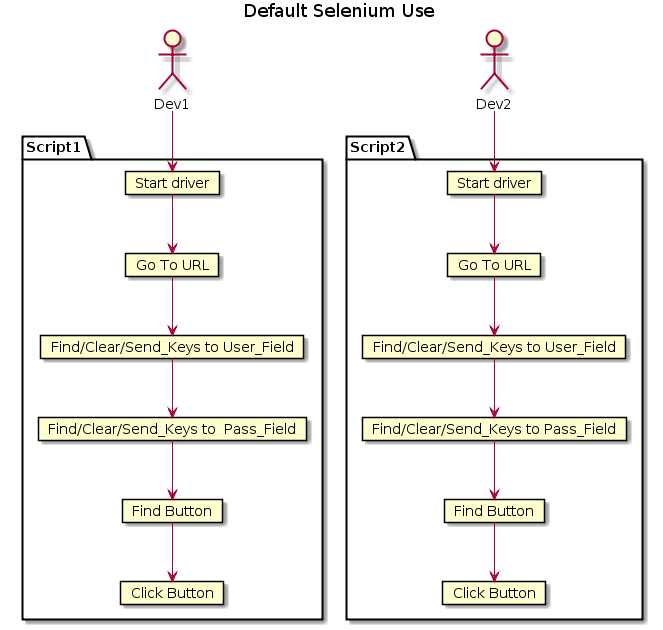
\includegraphics[width=0.8\textwidth]{./04-figuras/page_object_selenium}
        \label{fig:selenium_default}
    \end{figure}

    \clearpage

    Num segundo exemplo poderíamos separar o \emph{script} de login e criar um módulo separado para ele. Desse jeito
    os \emph{scripts} podem fazer uso do mesmo codigo e caso uma terceira pessoa precise dele não seria um problema.
    Porém temos todo o mapeamento dessa página preso num módulo e caso seja necessário a criação de outro
    módulo que use esses campos ainda assim teremos que duplicar mais codigo.

    \begin{figure}[H]
        \vspace*{0,3cm}
        \centering
        \caption{Uso padrão Selenium com módulo}
        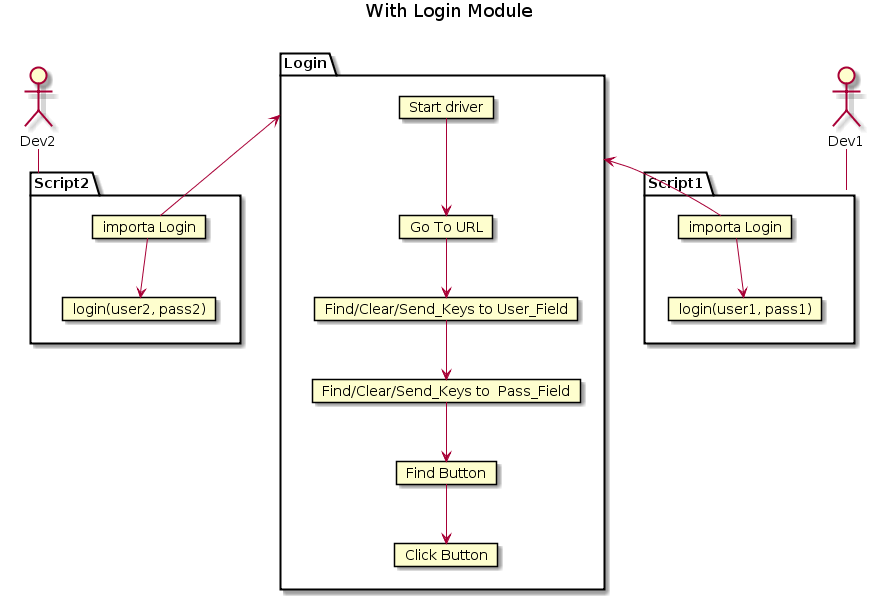
\includegraphics[width=1\textwidth]{./04-figuras/page_object_module}
        \label{fig:selenium_module}
    \end{figure}

    \clearpage
    Chegando num terceiro exemplo onde agora fazemos uso do framework \emph{Pybot}, onde utilizando-se do
    módulo Component(\ref{Comp}) podemos separar todos os componentes da tela em atributos da nossa página
    e criar um método onde precisando de dois parâmetros ele faz o processo de login, e ainda assim, caso
    necessário podemos ainda utilizar os campos mapeados para fazer algum outro método sem impactar o login.
    E caso alguma referencia dos campos mapeados mude, será necessário alterar apenas um local e nenhum \emph{script}
    será impactado.

    \begin{figure}[H]
        \vspace*{0,3cm}
        \centering
        \caption{Uso padrão Pybot}
        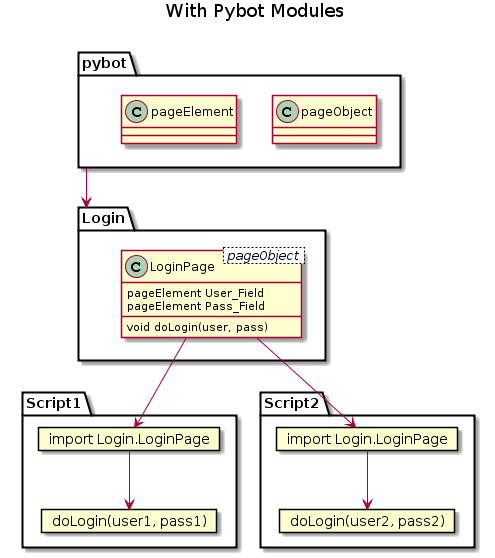
\includegraphics[width=0.8\textwidth]{./04-figuras/page_object_pybot}
        \label{fig:pybot_module}
    \end{figure}